\documentclass[a4paper,11pt,twoside,openright]{scrbook}

\usepackage{swThesis}
\usepackage{lipsum}
\usepackage{standalone}
\usepackage{caption}
\standalonetrue

% Bibliography
\bibliography{bibliography}

% Figures
\graphicspath{./figs}

\begin{document}

\chapter{Introduction} \label{chapter:intro}


\section{Eroom's Law: The increasing cost of drug discovery}
Throughout the last 70 years the cost of developing a new drug has steadily increased.
A study by Scannel \textit{et al.} noted the cost to develop a new drug has approximately doubled every 9 years, \cite{Scannell2012} this observation has been dubbed ``Eroom's law'', a homage to Moore's law -- the well-known observation that the number of transistors in microprocessors approximately doubles every 2 years.
The cost of bringing a new drug to market is now approaching £1 billion, taking 10 years from initial concept to approval, the reasons behind this every-increasing cost are still very much in debate, though most agree the issue is multi-faceted.
One explanation may be that the low-hanging fruit has been taken, effective traditional remedies have been studied and their active ingredients commercialised, natural products screened, leaving us to tackle the more complex diseases and pharmacological targets.  
This pessimism has led to the ever present idea that drug discovery is undergoing a productivity crisis, and that the investments made in early stage research do not translate into actionable pharmacology which can be used to develop efficacious therapies and ultimately benefit patients.
This belief has led to a renewed interest in alternative drug discovery paradigms.

% perceived decrease in productivity, leading to increased interest in other
% drug discovery paradiagms.
% lots of interest in diverse approaches to drug-discovery
% incorporate more technology intro drug-discovery

\section{The drug discovery process}

% Typically, commercial drug discovery programmes follow a well-established sequence of events, starting with selecting a disease or indication
% \begin{enumerate}
%     \item For a given disease or indication, an assay is developed which allows for high-throughput screening of large chemical libraries.
%     \item Hits are selected based on a univariate read-out. These are then confirmed with further repeats.
%     \item Lead compounds are then validated by testing in more complex assays, such as \textit{in vitro} or \textit{in vivo} disease models.
%     \item Validated compounds are taken through DMPK and toxicity testing.
%     \item A lead compound is selected and taken onto clinical trials.
%         \begin{enumerate}
%             \item phase I: Toxicity and DMPK testing.
%             \item phase II: Effectiveness at treating the condition.
%             \item phase III: Larger scale testing of efficacy.
%         \end{enumerate}
% \end{enumerate}
% \texttt{why is this being written about??}


\subsection{Target-based screening}
Over the past 30 years the majority of drug discovery programmes have seized upon technological advances in robotics and automation to screen ever expansive compound libraries against pre-defined protein targets.
It would be difficult to argue that this target-based high-throughput screening (HTS) approach has not been fruitful, yielding many succesful therapeutics across a range of disease areas, largely attributed to an increased understanding of the genomic basis of many diseases.
However, despite numerous clinical and commerical success stories, HTS is not a panacea, with a high attrition rate of lead compounds once they enter clincial trials. \cite{citation_needed}
A large majority of these clinical trial failures are not due to toxicity, but rather a lack of efficacy which can often be traced back to a poorly hypothesised target in the face of complex disease aetiology.


% issues with prior identification of a target
% large gamble on the hypothesised target
% examples where this has failed - Alzheimers? neuroscience in general?

\subsection{Phenotypic screening}
Phenotypic screening differs from target-based screening in that it does not rely on prior knowledge of a specific target, but instead interrogates a biologically relevant assay to identify compounds which alter the phenotype in a biologically desirable way.
This target-agnostic approach can prove useful in diseases with poorly understood mechanisms, or those with no obvious druggable protein targets.
Phenotypic screening is not a new approach in small molecule drug discovery, it was the primary method for many decades before the genomics revolution made target hypothesis tractable.
\cite{Zheng2013}

An example of a modern day target-agnostic phenotypic screen is the development of the anti-hepatitis C drug daclatasvir.
A model was developed in which human cells were modified to express the hepatitis C virus (HCV) replicon, this was then screened to identify compounds which reduced HCV replication.
The target for daclatasvir was later found to be the HCV NS5A protein, which is a novel target and likely not have been suggested in a hypothesis-driven screen as at the time it was thought to have no involvement with HVC. \cite{Belema2014,Nettles2014}
This elegant assay has the very useful attribute of modelling the disease whilst simulatenously identifying compounds which may prove to be toxic in human cells.

Many concerns related to phenotypic screening are centered on the lack of mechanistic information for a given lead compound.
Whilst the lack of a known target may cause concerns within a commercial drug discovery programme, regulatory bodies such as the Food and Drug Administration (FDA) and European Medicines Agency (EMA) do not require a known target for drug approval -- only that it is safe and efficacious.
Metformin, a first-line therapy for type 2 diabetes, and is on the World Health Organisation's list of essential medicine, decreases liver glucose production and has a insulin senstitising effect on many tissues.
Despite approval since 1957 and widespread clinical use, the  molecular mechanism of metformin remained unknown for 43 years. \cite{Hundal2000}
Although knowledge of the molecular target is not necessary to get a drug into the clinic, target deconvolution is still an important part of phenotypic drug discovery programmes -- without knowing the protein or proteins a compound is binding to, lead optimisation via structure activity relationship (SAR) studies becomes extremely difficult.
In addition, knowledge of the molecular target of a lead compound generated by a phenotypic screen can be used as a basis for starting a more high-throughput hypothesis-driven screen on a novel target, this is why many view phenotypic screening as a complimentary method to target based screening rather than a competing approach or proposed replacement.

% resurgence in recent years -> swinney and anthony, first in class



\section{High content imaging}
High content imaging is a technique utilising high-throughput microscopes and automated image analysis, commonly used in phenotypic screening as a method for gathering multivariate datasets from images of biological specimens and has proven useful in a wide variety of phenotypic assays, ranging from 2D mammalian cells \cite{cite_HCA_cell_papers}, \textit{in vivo} studies in zebrafish \cite{GeoffreyBurns2005} and even plants and crops. \cite{Chen2014}

%TODO: how morphology captures a lot of information about the internal
%state of a cell
High content screens -- screening studies carried out with high content imaging -- are particularly useful in phenotypic drug discovery for a few reasons.
The first is that they allow the use of more complicated assays, which might better represent the biological complexity than simple reductionist models.
However, these complex assays often have readouts which are more difficult to quantify, which a single univariate readout may fail to accurately recapitulate,
therefore the multivariate datasets produced by high content screening enables a more detailed representation of a complex assay endpoint.
A second benefit is that the multivariate nature of the data generated by high content screening may offer a more unbiased method for detecting hits in a phenotypic assay, as any single variable chosen beforehand may miss biologically interesting phenotypes which were not predicted.

With the advent of more complex datasets generated from high-content imaging, the process of image-analysis and computational methods for data processing has given rise to the term ``high-content analysis''.


\subsection{Image analysis}
After images are generated in a high-content screen, image analysis is the process in which raw image data is transformed into measurements which can be used the describe the observed morphology of the biological specimen exposed to a perturbagen.
Here I will focus on cell-based assays for small-molecule screening, though the same methods apply for most other assays (spheroids/organoids etc) and perturbagens (siRNA, CRISPR etc).

% segmentation
The standard approach to extracting numerical features from cell morphologies is through segmentating cells and sub-cellular structures into ``objects'', and then computing image-based measurements on those objects.
Typically each cell within image is identified by first segmenting nuclei from the background.
A number of well-established image thresholding algorithms can be used for segmentating nuclei from background, most automatically calculate an intensity threshold to binarise an image based on histograms of pixel pixel intensities.\cite{Otsu1979,Padmanabhan2010}
The segmented nuclei can then be used as seeds to detect cell boundaries, either through edge detection in a channel containing a cytoplasmic marker, or more crudely by expanding a number of pixels from the nuclei center to approximate cell size.
There are also less commonly used methods which utilise machine learning to segment cells, \cite{Sommer2011} or forgo segmentation entirely. \cite{Rajaram2012,Orlov2008}

After cells and sub-subcelluar objects have been segmented morphological characteristics are measured for each object, these measurements can cover a wide variety of morphologies depending on the aims of the assay, although can be grouped into 4 main classes:

\begin{itemize}
    \item \textbf{Shape.} Calculated on the properties of the object masks, e.g. area, perimeter, eccentricity. Shape features are commonly used as they are interpretable, robust, and quick to calculate.
    \item \textbf{Intensity.} These features are based on the pixel intensity values within the object boundaries.
They can be calculated for multiple channels and include measurements such as average intensity, integrated intensity, and radial distribution of intensity values.
Great care has to be taken when using intensity values as they are susceptible to batch effects and microscope artefacts such as vignetting. \cite{Goldman2010}
    \item \textbf{Texture.} Measures of patterns of intensities within objects, typically measured using grey level co-occurance matrices. \cite{Haralick1973} 
This can be used to quantify morphologies such as small speckles or stripes from labelled actin filaments.
Texture measurements are often computationally expensive and difficult to interpret, although can be used to quantify subtle morphological changes.
    \item \textbf{Spatial context.} These are typically relationships between objects, such as the number of neighbouring cells or nuclei, percentage of a cell boundary in contact with neighbouring cells. This class can also include the simple measure of cell or nuclei count within a field of view.
\end{itemize}


\subsection{Data analysis}
Measuring morphological features produces an $m \times n$ dataset per object class, where $m$ is the number of objects and $n$ is the number of morpholgical features measure for that object.
Commonly single object level data is aggregated to population level, where the population can be a field of view, microtitre-well, or treatment level (see figure \ref{figure:aggregation}); with the most popular aggregation method being a simple median average. \cite{Caicedo2017}
Once the object-level data has been aggregated to a common population level such as per well data, the features from each object class can be combined into a dataset represented by a single $p \times q$ matrix, where $p$ is the number of wells (or other level of aggregation), and $q$ is the total number of combined features from all object classes.
It is then useful to view each row of this matrix as a feature vector, or morphological profile which summarises the morphology induced by a treatment.


\begin{figure}
    \captionsetup{width=0.8\textwidth}
    \caption[Single cell aggregation to a median profile]{Single cell data aggregation to a median profile. Two matrices representing single cell morphology data for a treatment, with columns displaying multiple measured morphological features for each cell represented as a row. \textit{(Figure re-used from Caicedo et al. Nat Methods, 2017)}}
    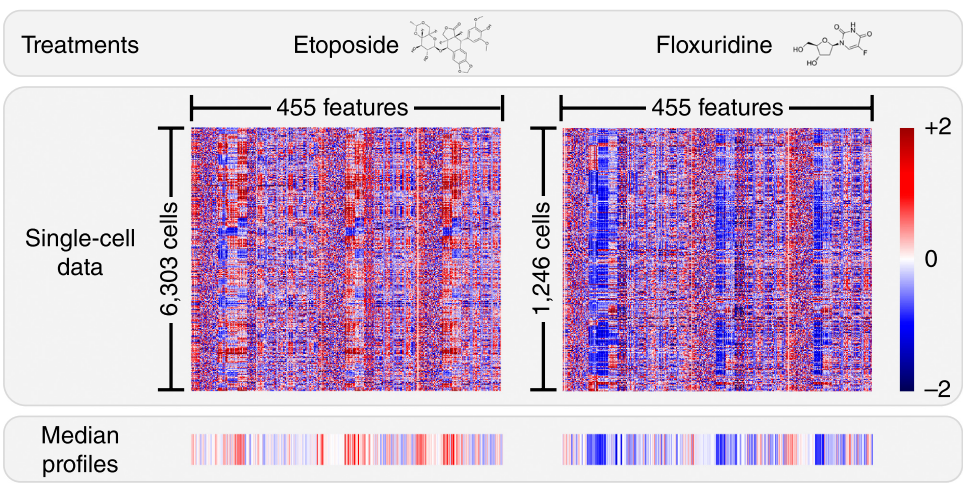
\includegraphics[width=0.8\linewidth]{figs/ch1SingleCellAggregation}
    \label{figure:aggregation}
\end{figure}


There are a number of fairly standard data pre-processing steps involved in high content analysis, consisting of: quality-control checks and outlier removal, batch correction, normalisation, standardising feature values, and dimensional reduction or feature selection. \cite{Caicedo2017}


\paragraph{\textbf{Quality control.}}
Errors are usually introduced at the imaging or segmentation phase of high-content assays, either through poor image quality caused by out-of-focus wells or debris, or otherwise acceptable images causing segmentation artefacts and subsequent outlier morphological features.
As assays often generate thousands if not millions of images it is not practical to manually check each image and segmentation mask, therefore a number of methods have been developed to flag potential image artefacts and extreme feature values.

Image artefacts can be detected through measures of image intensity, as out-of-focus images tend to have shallow intensity gradients across the image and lose high-frequency intensity changes. \cite{Bray2012}
Extreme feature values caused by segmentation errors fall into the well-researched field of outlier detection, with readily available methods such as Hampel filtering \cite{Hampel1974} or local outlier factor. \cite{Breunig2000}

\paragraph{Batch correction.}
Batch effects are accumulations of multiple sources of technical variation such as equipment, liquid-handling error, reagents and environmental conditions which can influence measurements and mislead researchers, and are particularly prevalent in high-throughput experiments.
They are normally identified by identifying visually through boxplots of features, with plates or weeks on the x-axis, or through comparing correlations, within plates, between plates of the same batch and across batches.
If batch effects need to corrected the simplist method is to standardise each batch separately, other methods include 2-way ANOVA \cite{Nygaard2016} or canonical correlation analysis. \cite{Vaisipour2014}

\paragraph{Standardisation.}
When many morphological features are measured from an image, they are unlikely to be in the same scale or have similar variation -- e.g. cell-area measured in pixels which may range from zero to several thousand and cell-eccentricity which is constrained between zero and one.
It is therefore common to standardize all feature values to be mean centered and have comparable variance.

\paragraph{Dimensional reduction and feature selection.}
As with any high-dimensional data a large number of features can cause issues with analysis and interpretation, this is commonly known as the ``curse of dimensionality''.
Another issue is that many of the measured features may not contribute information, either as they have little or no variation between samples, or are redundant due to high correlation with existing features.
Dimensional reduction and feature selection methods are both commonly used in other biological fields such as genomics and proteomics, and are now routinely used in high-content imaging analysis.
The most commonly used technique in principal component analysis (PCA), which is an unsupervised approach to maximise variation through a linear combination of orthogonal features.
PCA can be used to reduce the number of features by selecting a subset of principal components which explain a specified proportion of variance in the data.
Loss of interpretability of one of the issues caused by using PCA, and why some researchers favour feature selection methods which aim to retain feature labels, while still reducing dimensionality by removing uninformative features.
Many of the feature selection methods are supervised, which may not fit in with unbiased analyses, although Peng \textit{et al.} developed an unsupervised minimum-redudancy-maximum-relevancy (mRMR) feature selection method which has found use in high-content analyses. \cite{Peng2005}
\newline

Following data pre-processing, downstream analysis is typically focussed on one of two tasks: identifying hit compounds in a screen, or comparing the similarity of morphology profiles created by treatments -- both of which use distance as a metric, either comparing hits against a negative control, or treatments against one another respectively.


\subsection{Image based screening}

Phenotypic and image based screens can be used in traditional drug discovery roles whereby a compound library is screened a biologically relevant cell-based assay in order to identify compounds which produce a favourable phenotype.
These assays rely on either a positive control compound which is known to elicit the phenotype of interest, or a carefully designed assay in which a disease model is used to identify compounds which push the disease associated phenotype towards a healthy one.
An example of this is demonstrated by Gibson \textit{et al.}, \cite{Gibson2015} whereby they modeled cerebral cavernous malformation (CCM) using siRNA knockdown of the \textit{CCM2} gene in human primary cells, and screened small molecules to identify candidates which rescued the siRNA induced phenotype using fluorescent markers of the nucleus, actin filaments, and VE-cadherin cell-cell junctions.
Candidate compounds were then validated in an \textit{in vivo} mouse model, which lead to the ongoing pre-clinical development of 4-Hydroxy-TEMPO as a novel therapeutic for CCM.
% TODO informatics --> how these work?
% TODO example of a phenotypic screen looking for cmpd like pos control


\subsection{Image based profiling}
% TODO why, compound MOA prediction, toxicity, side-effects
In contrast to screening studies which are mainly interested in looking for a defined phenotype, profiling studies are used to create phenotypic ``fingerprints'' of perturbagens analogous to transcriptional profiles, which can be used for clustering, inference and prediction.
One of the main uses of phenotypic profiling to compare the similarity of morphological profiles, allowing clustering and machine learning methods to build rules in order to classify new or blinded treatments according to similar annotated neigbours.

One of the landmark papers of high-content imaging and profiling was published in 2004 when Perlman \textit{et al.} \cite{Perlman2004} first demonstrated that morphological profiles between drugs could be clustered according to compound mechanism-of-action using a custom similarity metric and hierarcical clustering.
Most studies utilising morphological profiling use unsupervised hierarchical clustering in order to group treatments into bins which produce similar cellular phenotypes, \cite{Gustafsdottir2013,Young2008} though other clustering algorithms such as graph-based Markov clustering algorithm (MCL), \cite{Reisen2015,VanDongen2008} and spanning trees \cite{Qiu2011} are commonly used.

% FIXME: not sure this paragraph is needed
An important component of profiling studies is the metric to compare similarity or distance between treatment profiles.
The choice of the distance or similarity metric is largely dependent on the dimensionality of the data and the intended downstream applications, although the distiction between distance and similarity is not important, as many similarity metrics and be converted to distances with $1 - \text{similarity}$.
A comparative study of similarity measures in high-content fingerprints found that rank-based nonlinear Spearman and Kendall correlations performed the best when comparing full-length
\footnote{Full-length meaning complete morphological profiles that have not been subjected to dimensionality reduction or feature selection methods.}
fingerprints. \cite{Reisen2013}


\section{Phenotypic screening in cancer drug discovery}
Cancer drug discovery programmes of past decades seized upon uncontrolled proliferation as a clinically relevant phenotype to screen against, giving rise to a number of anti-proliferative and cytotoxic compounds, often renowned for their severe side-effects.
Many modern day oncology drug discovery programmes still retain anti-proliferation as a key predictor for pre-clinical success, although our ever increasing understanding of cancer's molecular underpinnings has driven many oncology programmes towards a more target-directed approach.
The prototypical success story of target-driven drug discovery in oncology is imatinib, a tyrosine kinase inhibitor targetting the BCR-ABL fusion protein in chronic myeloid leukemia.
However, despite imatinib's exceptional success, it is unfortunately very much an exception -- in most cases targeting a single driver in a complex signalling network results in compensatory signalling, activation of redundant pathways and unpredicted feedback mechanisms, all of which diminish efficacy \textit{in vivo}.

In a review of 48 small molecule drugs approved for use in oncology between 1999 and 2013, $31/48$ were discovered through target based screens, whereas $17/48$ were based on leads from target-agnostic phenotypic screens, \cite{Moffat2014} of those compounds discovered through target directed screening programmes the vast majority (75\%) were kinase inhibitors.
However phenotypically derived compounds did not live up to the hypothesis that target-agnostic screening should be more likely to identify compounds with novel MoAs, \cite{Swinney2011} with only $5/17$ being first in class molecules.
An explanation for this sparsity of novel mechanisms is that phenotypic assays which use cytotoxicity readouts are likely to find low-hanging fruit such as targetting microtubule stabilisation and DNA replication dynamics. \cite{Moffat2014}
One option to combat this narrow attention on a select few targets -- caused by either hypothesis-driven or simplistic phenotypic screens -- is to utilise the more detailed mechanistic information offered by high-content imaging rather than relying on cellular death as catch-all phenotypic readout.

In addition to 2D high-content imaging screens, more complex phenotypic models such as 3D tumour spheroids are becoming increasingly prevelent in preclinical oncology, much of this stems from the hypothesis that they better recapitulate the microenviroment found in tumours.
%TODO: more complex phenotypic models to better recapitulate the biology -> tumour spheroids

\subsection{Cancer cell line panels}
Panels of multiple cancer cell lines such as the NCI-60 and Cancer Cell Line Encyclopedia (CCLE) have been widely used; initially to facilitate high-throughput screening and increase certainty in hit selection/disease-specificity \cite{Wu1992,Shoemaker2006}, and later on as a research tool to study pharmacogenomics. \cite{Heiser2012,Abaan2013,Jaeger2015}
The use of cancer cell line panels can also benefit phenotypic screens by mirroring the heterogeniety found in patient populations, as well as heterogenous cell populations found in tumours \cite{Caie2010}.
Throughout this body of work I have used a panel of eight breast cancer cell lines (table \ref{table:cell-lines}), these cell lines were chosen based on a number of criteria:
\textit{(1)} Relatively fast growth to allow compound screening to be performed in weekly batches.
\textit{(2)} Adherent to tissue culture plastic to enable 2D imaging.
\textit{(3)} Form a monolayer when grown in 2D -- overlapping cells cause difficulties for most image segmentation methods.
\textit{(4)} Amenable for imaging -- larger and/or flatter cells allow for better discrimination of sub-cellular features.
\textit{(5)} Distinct morphologies to evaluate the robustness of morphological profiling methods.
\textit{(6)} A collection which represents a range of molecular subclasses of breast cancer.

\begin{table}[]
    \begin{footnotesize}
    \captionsetup{width=0.8\linewidth}
    \centering
    \caption[Panel of breast cancer cell lines chosen for study]{Panel of breast cancer cell lines chosen for study. PI3K:Phosphoinsitide-3-kinase, PTEN:Phosphatase and tensin homolog, ER:Estrogen receptor, TN:triple-negative, HER2:human epidermal growth factor, WT:wild-type, $\star$:lack of consensus regarding the mutational status.}
    \label{table:cell-lines}
    \begin{tabular}{@{}llll@{}}
    \toprule
               &                    & \multicolumn{2}{l}{Mutational status} \\
    Cell line  & Molecular subclass & PTEN             & PI3K               \\ \midrule
    MCF7       & ER                 & WT               & E545K              \\
    T47D       & ER                 & WT               & H1047R             \\
    MDA-MB-231 & TN                 & WT               & WT                 \\
    MDA-MB-157 & TN                 & WT               & WT                 \\
    HCC1569    & HER2               & WT               & WT                 \\
    SKBR3      & HER2               & WT               & WT                 \\
    HCC1954    & HER2               & $\star$          & H1047R             \\
    KPL4       & HER2               & $\star$          & H1047R             \\ \bottomrule
    \end{tabular}
    \end{footnotesize}
\end{table}

\section{Thesis structure}
The following chapters focus on selected topics from 4 years of work, some of which has been published (see appendix).
Chapter 2 is an analysis of machine learning methods to classify compound MoA from high content imaging data, with a focus on how well classifiers transfer across to new data from morphologically distinct cell lines.
Chapter 3 is the development and application of a novel analytical method to detect and quantify differential phenotypic responses between morphologically distinct cell lines when treated with small molecules.
Chapter 4 is a high content screen of 13,000 small molecules in order to identify compound that produced distinct phenotypic responses between cell lines, functional assays to validate hits and proteomics to investigate potential pathways responsible.
Chapter 5 is a work towards combining cheminformatics with high content morphological data in order to infer MoA of unannotated compounds.


%\printbibliography

\end{document}
